\section{Aluminiumoxid-ALD}
\label{aluminaald}

Einen Vorzeige-Prozess für Atomlagenabscheidungen bildet die Abscheidung von Aluminiumoxid \ce{Al2O3}\cite{puurunen_surface_2005}, für die häufig das Precursorpaar Trimethylaluminium (TMA, \ce{Al(CH4)3}) und Wasser genutzt wird.
Mit einer Permittivität von $k\approx 8$ ersetzt Aluminiumoxid gemeinsam mit anderen Materialien langsam Siliziumdioxid ($k=3.9$) als Dielektrikum in der Halbleiterindustrie.
Deshalb soll der TMA-\ce{H2O}-Prozess im Folgenden besonders hinsichtlich der Reaktion der Precursormoleküle mit der Oberfläche untersucht werden.
Einige Reaktionen des Wasser-Halbzyklus' konnten dabei erfolgreich simuliert werden, wo hingegen die Simulation des TMA-Halbzyklus' bisher keinen Erfolg zeigte.

\subsection{Parametersätze}

Für die MD-Simulation von \ce{Al2O3} stehen drei Parametrisierungen zur Verfügung, die bereits aus den Untersuchungen der Silizium-Potentiale bekannt sind:\\
\textbf{Al\_AlO\_AlN} aus LAMMPS\cite{plimpton_lammps_2014}, \textbf{liu\_ettringite}\cite{liu_development_2012}, welches nachfolgend nur als \textbf{liu} geführt werden soll, und \textbf{narayanan}\cite{narayanan_reactive_2012}.
Ihnen ist gemein, dass sie ausgehend von Silizium-kompatiblen Potentialen um Parameter für Aluminium-Verbindungen erweitert wurden.
Auf eine Bewahrung der Konsistenz der Siliziumparameter wurde scheinbar verzichtet, so dass etwa mit der Liu-Datei eine verlässliche Simulation von  Silizium-Verbindungen verhindert, im Gegenzug aber die Simulation von Aluminium-Verbindungen ermöglicht wird.

Die Al\_AlO\_AlN-Datei stammt direkt aus der offiziellen LAMMPS-Distribution, wurde jedoch am 17. Mai 2013 nahezu kommentarlos aus dem Paket entfernt, was sich vermutlich auf mangelnde Kenntnis der Urheberschaft der Parameter sowie ihrer Zielsetzung zurückführen lässt.
Diese Vermutung wird von der Überarbeitung der Referenzen auf wissenschaftliche Publikationen für alle Parametersätze im selben Zeitraum gestützt.
Bei den Recherchen konnte kein Hinweis auf das ursprüngliche Anwendungsgebiet gefunden werden, weshalb mit diesen Parametern berechnete Eigenschaften gesondert überprüft werden sollten.
Es lässt sich jedoch sagen, dass es zeitgleich mit dem \textbf{lg}-Kraftfeld, welches sich bei den Silizium-Untersuchungen als unzureichend heraus gestellt hat, Eingang in LAMMPS gefunden hat.

Das Anwendungsgebiet der Liu-Potentialdatei liegt in der Simulation von Ettringit (\ce{Ca6[Al(OH)6]2(SO4)3 26H2O}), welches \ce{Al-O}-Bindungen und \ce{OH}-Gruppen enthält, so dass zumindest die Simulation des Bulkmateriales und einer hydroxylierten Oberfläche aussichtsreich erscheint.
Sie unterstützt einige der Precursorreaktionen und stellt sich daher als Favorit für Parsivald-Simulationen heraus, obwohl ihr eigentliches Anwendungsgebiet auf strukturellen Eigenschaften von Kristallen liegt.

Zuletzt steht die Narayanan-Parametrisierung für \ce{Li-Al}-Silikate für die Simulation von Eukryptit (\ce{LiAl[SiO4]}) zur Verfügung, lässt aber keine endgültige Aussage über die Qualität der \ce{Al-O}-Bindungen und \ce{OH}-Gruppen zu.
Zwar besteht ihr Trainingssatz aus verschiedenen Lithium-Aluminium-Kristallen, aber nur $\gamma$-\ce{LiAlO2} beinhaltet direkte \ce{Al-O}-Bindungen, wo hingegen keine der Strukturen Wasserstoff beinhaltet.
Es ist daher unwahrscheinlich, dass die Narayanan-Potentialdatei komplizierte Systeme verlässlich darstellt.

Abschließend lässt sich sagen, dass zur vollständigen Simulation der untersuchten Systeme die Erstellung einer eigenen Parametrisierung notwendig wäre, die jedoch den Fokus dieser Arbeit übersteigt.

\subsection{Voruntersuchungen}

Wie in den vorherigen Abschnitten werden hier separate Voruntersuchungen durchgeführt, zu denen die Reaktion von Precursormolekülen mit der Oberfläche ergänzt wurde.

\subsubsection{Strukturelle Eigenschaften von \ce{Al2O3}}

Zum Vergleich der strukturellen Eigenschaften des Bulkmateriales, wie etwa Dichte, Bindungslänge und Koordinationszahlen, wurde ein $\alpha$-\ce{Al2O3}-Kristall bei \SI{1500}{\kelvin} relaxiert und vor den abschließenden Messungen auf Raumtemperatur herunter gekühlt.
Durch einen methodischen Fehler wurden die Systeme zur Dichtebestimmung nicht vollends herunter gekühlt, weshalb die Referenzwerte anhand der Relaxationstemperatur korrigiert wurden.
Damit ergibt sich ein korrigierter Referenzwert zwischen \SI{3.95}{\gpcc} bei \SI{300}{\kelvin} und \SI{3.8}{\gpcc} bei \SI{1500}{\kelvin}\cite{fiquet_high-temperature_1999}, der im direkten Vergleich als \SI{3.85}{\gpcc} abgeschätzt wird.
Der dadurch entstehende Fehler ist im Vergleich zu Abweichungen um \SI{0.5}{\gpcc} gering.

Für die Bestimmung der Dichte der amorphen Struktur wurde das Bulkmaterial über den Schmelzpunkt von \SI{2317}{\kelvin} auf \SI{2555}{\kelvin} erhitzt, auf dieser Temperatur relaxiert und langsam auf Raumtemperatur abgekühlt.
Aufgrund der strukturellen Vielfalt bei amorphen Aluminiumoxiden lässt sich keine eindeutige Referenzdichte angeben, so dass auf den in diesem Zusammenhang häufig genannten Wertebereich von \SIrange{3.2}{3.6}{\gpcc} zurückgegriffen wurde.

Bindungslängen und Koordinationszahlen wurden direkt aus der radialen Verteilungsfunktion bestimmt, wobei die Referenzwerte auf gleiche Weise durch die Untersuchung der Kristallstruktur bestimmt wurden, welche mittels Materials Studio auf Basis eines $\alpha$-\ce{Al2O3}-Kristalles präpariert wurde.

\begin{table}
  \caption[Vergleich struktureller Eigenschaften von Bulk-\ce{Al2O3} mit verschiedenen Parametersätzen]{
    Vergleich struktureller Eigenschaften von Bulk-\ce{Al2O3} mit verschiedenen Parametersätzen.
    Bindungslängen und Koordinationszahlen stammen von einer relaxierten Kristallstruktur.
  }
  \label{tab:aluminabulks}

  \begin{tabularx}{\textwidth}{|Xllll|}
    \hline
    \textbf{Eigenschaft}    & \textbf{Referenz}    & \textbf{Al\_AlO\_AlN} & \textbf{liu}         & \textbf{narayanan}   \\
    \hline
    Dichte, amorph          & \SI{>3.2}{\gpcc}     & ~                     & \SI{3.66}{\gpcc}     & ~                    \\
    Dichte, kristallin      & \SI{3.85}{\gpcc}     & \SI{4.31}{\gpcc}      & \SI{3.88}{\gpcc}     & \SI{3.76}{\gpcc}     \\
    \ce{Al-O}-Bindungslänge & \SI{1.90}{\angstrom} & \SI{1.94}{\angstrom}  & \SI{1.88}{\angstrom} & \SI{1.85}{\angstrom} \\
    \ce{Al-O}-Koordination  & \num{4.00}           & \num{5.40}            & \num{4.55}           & \num{4.05}           \\
    \ce{Al-Al}-Koordination & \num{4.00}           & \num{6.66}            & \num{5.98}           & \num{5.10}           \\
    \ce{O-O}-Koordination   & \num{12.0}           & \num{12.4}            & \num{11.0}           & \num{12.2}           \\
    \hline
  \end{tabularx}
\end{table}

Die Ergebnisse dieser Untersuchungen (Tabelle~\ref{tab:aluminabulks}) zeichnen ein vielseitiges Bild.
Einerseits stimmen die Bindungslängen für alle Parametrisierungen auf \SI{2}{\percent} überein, andererseits ergeben sich aber große Unterschiede in der Dichte der Kristalle, die sich nicht mit den Bindungslängen korreliert sind.

So liegt für die Al\_AlO\_AlN-Parameter eine Abweichung um \SI{+12}{\percent} in der Dichte vor, allerdings ist die Bindungslänge um \SI{2}{\percent} erhöht, was für ähnliche Strukturen zu einer Ausdehnung des Kristalles und somit eine Verringerung der Dichte um \SI{6}{\percent} führen müsste.
Erst bei Betrachtung der Koordinationszahlen zeigt sich die Ursache der Abweichung, die mit einer \ce{Al-O}-Koordinationszahl von \num{5.4} (Kristall: \num{4.0}) in einer Verformung des Kristalles liegt.
Da $\alpha$-\ce{Al2O3} mit \SI{3.95}{\gpcc} eigentlich die dichteste Phase bei Normaldruck ist, sollten nur Übergänge zu weniger dichten Konfigurationen wie amorphem Aluminiumoxid oder etwa $\gamma$-\ce{Al2O3} möglich sein, das aufgrund seiner Porösität eine geringere Dichte von etwa \SI{3.67}{\gpcc}\cite{dynys_alpha_1982} aufweist.
Da hier das Gegenteil der Fall ist, wurde die Al\_AlO\_AlN-Parameterdatei in vielen der nachfolgenden Untersuchungen nicht weiter betrachtet.

Die Liu-Parametrisierung weist ebenfalls eine geringe Änderung aller Koordinationszahlen auf, die sich in einer nur minimalen Verringerung der Dichte äußert.
Anhand einer \ce{Al}-{O}-Koordination von \num{4.55} ist ersichtlich, dass die $\alpha$-Phase mit diesem Parametersatz nicht stabil ist und stattdessen scheinbar eine vergleichsweise dichte amorphe Phase angenommen wird.
Für diesen Parametersatz wurde deshalb auch die Dichte eines amorphen Materiales mit \SI{3.66}{\gpcc} bestimmt, die zwar innerhalb des üblicherweise für amorphe Materialien genannten Bereiches von \SIrange{3.2}{3.6}{\gpcc} liegt, ansonsten aber unterhalb der im ersten Schritt bestimmten Dichte liegt, womit eine höhere Porösität denkbar wird.

Zum Schluss zeigt Die Narayanan-Parameterdatei die besten Ergebnisse für kristalline Strukturen, obwohl sowohl die Bindungslänge als auch die Dichte ca. \SI{2}{\percent} unterhalb der jeweiligen Referenzwerte liegen.
Dies ist im Zusammenhang mit dem Fehlen von \ce{Al-O}-Bindungen in den meisten Molekülen des Trainingssatzes eher überraschend, zeigt aber die Orthogonalität der einzelnen ReaxFF-Parameter, da so die Eigenschaften von $\gamma$-\ce{LiAlO2} die \ce{Al-O}-Bindungen dominieren, statt beim Fitting überschrieben zu werden.

\subsubsection{Precursor-Simulationen}

Zur Untersuchung der Stabilität der Precursor wurden diese einzeln präpariert und per LAMMPS mit verschiedenen Kraftfeldern im kanonischen Ensemble simuliert.
Dabei war schnell ersichtlich, dass Trimethylaluminium (TMA) von der Liu- sowie der Narayanan-Parametrisierung in Ermangelung der Ausprägung von \ce{Al-C}-Bindungen praktisch nicht simuliert werden kann.
Die Methylgruppen binden nicht mit dem zentralen Aluminium-Atom, so dass sie sich von diesem mit fortlaufender Simulationszeit linear entfernen.
Einzig mittels des bereits ausgeschlossenen Al\_AlO\_AlN-Parametersatzes lassen sich stabile TMA-Moleküle simulieren.

\todo[inline]{Bilder im Anhang}

Simulationen von Wassermolekülen sind hingegen mit allen Parametrisierungen geglückt, doch wurden keine umfangreicheren Untersuchungen etwa hinsichtlich der Phasenübergänge angestellt.
Anhand des Al\_AlO\_AlN-Parametersatzes wurden auch Reaktionen zwischen TMA und Wasser simuliert, wie sie beispielsweise bei Vermischung der Precursorgase im ALD-Reaktor auftreten können, aber \todo{phrasing}leider ohne Erfolg.
Es zeigt sich, dass die \ce{Al-C}-Bindungen entweder zu stark oder in zu großem Maß von den Methylgruppen abgeschirmt sind.

\subsubsection{Precursor-Oberflächen-Reaktionen}

Anstatt die Precursormoleküle in der Gasphase reagieren zu lassen, werden hier einzelne Wassermoleküle auf eine $\alpha$-\ce{Al2O3}-Kristalloberfläche gebracht, die mit den darauf befindlichen Sauerstoffatomen reagieren und die Oberfläche so hydroxylieren sollen\todo{Ref}.
Zu diesem Zweck wurde ein mehrschichtiges System mit einem kristallinen Substrat und einer Schicht von Wassermolekülen in Gasphase präpariert, wie es in Abbildung~\ref{fig:wateraluminasurface-a} dargestellt ist.
In der Simulation werden die Wassermoleküle mit einer maxwellschen Geschwindigkeit entsprechend \SI{500}{\kelvin} versehen, die Atome an der Unterseite des Substrates fest gehalten und das Berendsen-Thermostat auf den verbleibenden Teil des Substrates angewandt.
Damit handelt es sich zwar streng gesehen nicht mehr um eine Simulation im kanonischen Ensemble, aber man verzichtet auf separate Integratoren für Substrat (NVT) und Wasser (NVE), deren Grenzen bei erfolgreichen Reaktionen ohnehin aufgelöst werden.

\begin{figure}
  \captionsetup[subfigure]{singlelinecheck=false}
  \def\subfigwidth{0.32\textwidth}
  \begin{subfigure}[t]{\subfigwidth}
    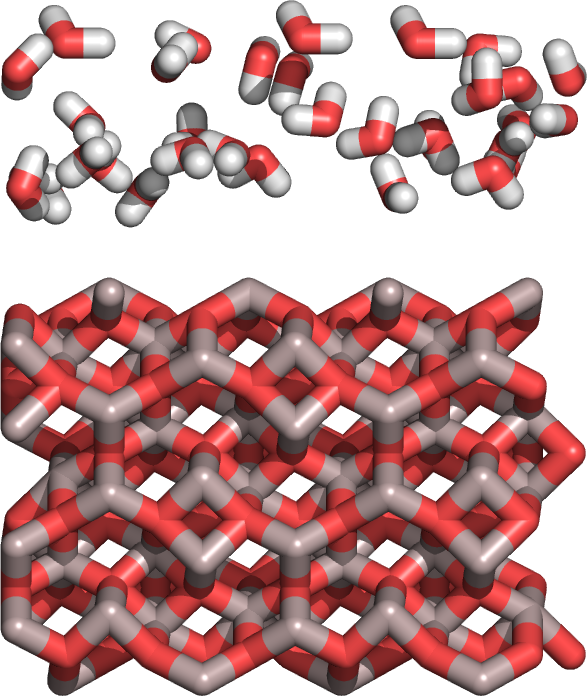
\includegraphics[width=\textwidth]{alumina_h2o_before}
    \subcaption{Seitenansicht, vorher}
    \label{fig:wateraluminasurface-a}
  \end{subfigure}
  \hfill
  \begin{subfigure}[t]{\subfigwidth}
    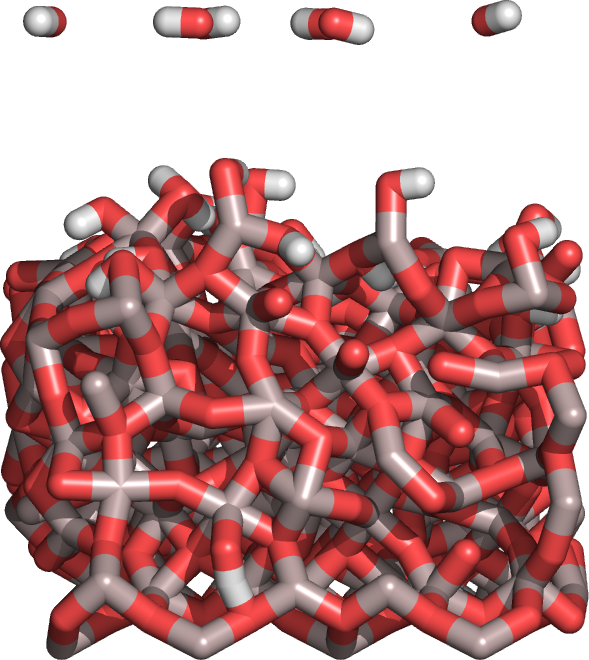
\includegraphics[width=\textwidth]{alumina_h2o_after}
    \subcaption{Seitenansicht, nachher}
    \label{fig:wateraluminasurface-b}
  \end{subfigure}
  \hfill
  \begin{subfigure}[t]{\subfigwidth}
    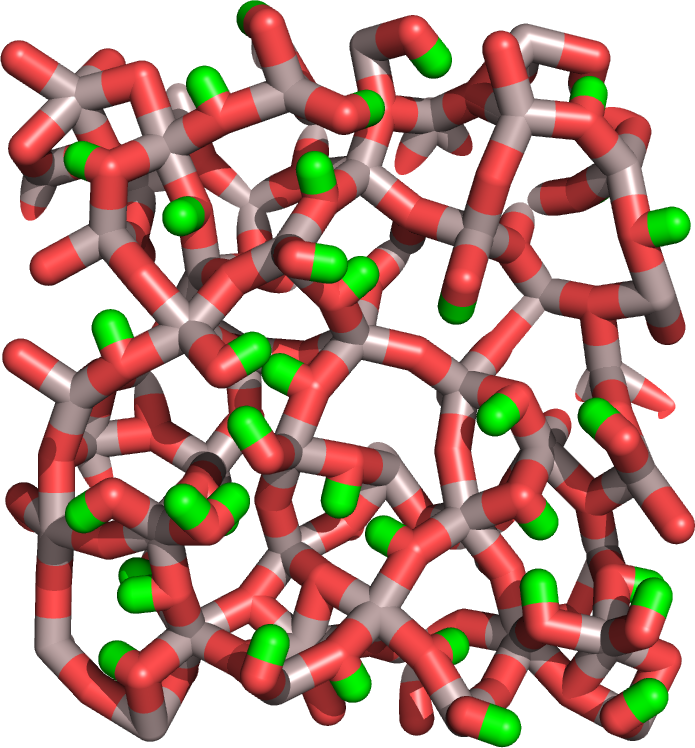
\includegraphics[width=\textwidth]{alumina_h2o_topview}
    \subcaption{Draufsicht, nachher.
      Hydroxyl ist grün hervorgehoben.
    }
    \label{fig:wateraluminasurface-c}
  \end{subfigure}
  \caption[Oberflächenreaktion von Wasser mit $\alpha$-\ce{Al2O3}]{Ergebnisse einer Oberflächenreaktion von Wasser mit $\alpha$-\ce{Al2O3}.
    Das Wasser reagiert mit Sauerstoffatomen an der Oberfläche zu Hydroxylgruppen.
  }
  \label{fig:wateraluminasurface}
\end{figure}

Das Ergebnis der Simulationen für die Liu-Parameter (Abbildungen~\ref{fig:wateraluminasurface-b} und~\ref{fig:wateraluminasurface-c}) zeigt die gleichmäßige Bedeckung der Oberfläche mit Hydroxylgruppen (\todo{tatsächlicher Wert!}\SI{19}{\per\square\nano\meter}) neben gelegentlich adsorbierten Wassermolekülen, die keine Oberflächenreaktion eingegangen sind.
Letztere sollten aber auf längere Sicht durch die Einflüsse der Überkoordinationsterme des ReaxFF-Potentiales entweder zerfallen oder sich von der Oberfläche lösen.
Trotz unterschiedlicher Startbedingungen stimmt der maximale Bedeckungsgrad der Oberfläche mit Hydroxylgruppen mit experimentell bestimmten Werten von \todo{eigentlicher Wert}\todo{Ref!}\SI{19}{\per\square\nano\meter} überein.
Zu Beginn der Simulationen wurden ausreichende Mengen von Wassermolekülen für Bedeckungsgrade von \todo{tatsächliche Werte!}\SI{20}{\per\square\nano\meter}, \SI{50}{\per\square\nano\meter} und \SI{100}{\per\square\nano\meter} präpariert, von denen die überschüssigen Moleküle im Verlauf der Simulationen stets in der Gasphase verblieben sind, wie in Abbildung~\ref{fig:wateraluminasurface-b} am oberen Rand des periodischen Simulationsraumes erkennbar ist.
Einige der Wassermoleküle sind durch periodische Randbedingungen des Simulationsraumes zerteilt, weshalb es sich scheinbar um Hydroxylmoleküle handelt, tatsächlich aber komplette Wassermoleküle verbleiben.
Es zeigt sich also die sterische Hinderung der Wasserstoffmoleküle gegenüber weiteren Reaktionen von Wasser mit der Oberfläche.

Eine repulsive Kraft zwischen den Wassermolekülen und der Oberfläche verhindert diese Reaktionen unter Nutzung der Narayanan-Parameter.
Das deutet darauf hin, dass Hydroxylgruppen auf einer Aluminiumoxid-Oberfläche energetisch nicht bevorzugt werden oder die Reaktion mit einer hohen Reaktionsbarriere verbunden ist.
Zusammen mit dem Problem, Trimethylaluminium nicht darstellen zu können, ist dieser Parametersatz somit nicht in der Lage, den ALD-Prozess darzustellen.

\todo[inline]{Hinweis auf vollständige ALD-Simulationen?}
\todo[inline]{Welche der alten Ergebnisse finden hier Anwendung?}
